\documentclass[aspectratio=169,11pt]{beamer}

\usetheme{Boadilla}
\usefonttheme{serif} % default family is serif
\usepackage[T3,T1]{fontenc}
\DeclareSymbolFont{tipa}{T3}{cmr}{m}{n}
\DeclareMathAccent{\invbreve}{\mathalpha}{tipa}{16}

\definecolor{robertsblue}{rgb}{0.27, 0.27, 0.67}

\setbeamercolor{title in head/foot}{bg=robertsblue}

% change footer information, including email address
\makeatother
\setbeamertemplate{headline}
{
  \leavevmode%
  \hbox{%
  \begin{beamercolorbox}[wd=1.0\paperwidth,ht=2.25ex,dp=1ex,center]{}%
  \usebeamerfont{title in head/foot} 
  \end{beamercolorbox}}%
  \vskip0pt%
}
\setbeamertemplate{footline}
{
  \leavevmode%
  \hbox{%
  \begin{beamercolorbox}[wd=1.0\paperwidth,ht=3.25ex,dp=2ex,center]{}%
  \usebeamerfont{author in head/foot} \color{gray} Variational Ridging in Sea Ice Models | Andrew Roberts | afrobert@nps.edu
  \end{beamercolorbox}}%
  \vskip 2pt%
}

\makeatletter
\setbeamertemplate{navigation symbols}{}

% left/center frame titles
\setbeamertemplate{frametitle}[default][center]

% change table of contents information
\setbeamertemplate{section in toc}{\hspace*{1em}\inserttocsectionnumber.~\inserttocsection}
\setbeamertemplate{subsection in toc}{\hspace*{2em}\inserttocsubsection}

% Mathematics typesetting
\usepackage{amsmath}
\DeclareMathOperator{\arcsec}{arcsec}
\DeclareMathOperator{\arccot}{arccot}
\DeclareMathOperator{\arccsc}{arccsc}
\usepackage{amsfonts}
\usepackage{mathtools}
\usepackage{textcomp}
\usepackage{units}
\usepackage{xcolor}
\usepackage{cancel}

% Diagram
\usepackage[absolute,overlay]{textpos}
\usepackage{tikz}
\usepackage{verbatim}
\usetikzlibrary{arrows,shapes,backgrounds,calc,positioning}
\usepackage{pgfplots}
\usepackage{filecontents}

% Figures and Tables 
\usepackage{graphicx}
\usepackage{epsfig}
\usepackage{epstopdf}
\epstopdfsetup{update}
\usepackage{subfig}
\usepackage{multimedia}

% bibliography
\usepackage{natbib}

% change itemize bullet points
\setbeamertemplate{itemize items}[circle]

% change font size
\newcommand\Fontvi{\fontsize{9}{7.2}\selectfont}

% set up title page
\setbeamercolor{title}{fg=white}
\title{\huge Variational Ridging in Sea Ice Models}
\subtitle{\vspace{3.5cm}}
\setbeamercolor{author}{fg=white}
\author{Andrew Roberts \vspace{-0.4cm}}
\setbeamercolor{institute}{fg=white}
\institute{Naval Postgraduate School\vspace{-0.28cm}}

% add date or leave empty as required
\setbeamercolor{date}{fg=white}
\date{\scriptsize{Elizabeth Hunke, Samy Kamal, William Lipscomb, Wieslaw Maslowski}\vspace{-0.4cm}}

% insert workshop in here
\addtobeamertemplate{title page}{}
 {\begin{center}\color{black}\tiny{C23E: Integrating Observations and Models to Better Understand a Changing Arctic Sea Ice Cover \\ 
 \textit{Fall AGU, New Orleans, 12 December, 2017}
 }\end{center}}


% path diagram (a plane with varying y coordinate)
\newcommand{\planemaina}[3]{
	(-2, #1, 2) --
	++(8, 0.3, 0) --
	++(0, -5, -8) --
	++(-8, -0.3, 0) --
	cycle;
	\node[fill=white,inner sep=2pt, anchor=east] at (-2, #1, 2) {#2};
	\node[anchor=north, black!40] at (5.8, #1+0.2, 5.5) {#3};
	}
	
\newcommand{\planemainb}[3]{
	(-2, #1, 2) --
	++(8, 0.3, 0) --
	++(0, -5, -8) --
	++(-8, -0.3, 0) --
	cycle;
	\node[fill=white,inner sep=2pt, anchor=east] at (-2, #1, 2) {#2};
	\node[anchor=north, orange!85] at (4.78, #1+0.3, 2.8) {#3};
	}

\newcommand{\planelittlea}[1]{
	(-0.2, #1, 2) --
	++(1.36, 0.126, 0) --
	++(0.24, -1.68, -2.7) --
	++(-1.45, -0.156, 0) --
	cycle;
	}
	
\newcommand{\planelittleb}[1]{
	(6.7, #1, 2) --
	++(1.1, 0, 0) --
	++(0, -1.4, -1.8) --
	++(-1.3, -0, 0) --
	cycle;
	}
	
\newcommand{\planelittlec}[1]{
	(1.9, #1, 2) --
	++(0.85, 0.026, 0) --
	++(0, -1.08, -1.8) --
	++(-0.85, -0.026, 0) --
	cycle;
	}

%%%%%%%%%%%%%%%%%%%%%%%%%%%%%%%%%%%%%%%%%%%%%%%%%%%%%%%%%%%%%%%%%%%	
\begin{document}

% remove "figure" from caption and (a) from caption
\setbeamertemplate{caption}{\raggedright\insertcaption\par}
\captionsetup[subfigure]{labelformat=empty,justification=centering}
\captionsetup[figure]{labelformat=empty,justification=centering}

% box seperation
\fboxsep=0pt

% title page and table of contents, centering for 
{
\usebackgroundtemplate{
\parbox[c][\paperheight][c]{\paperwidth}{\centering\includegraphics[width=\paperwidth]{Figures/SEDNA_site1_3_20070409054800.jpg}}
}
\setbeamertemplate{headline}{}
\setbeamertemplate{footline}{}
\begin{frame}[t,fragile]
\titlepage
\end{frame}
}

%%%%%%%%%% section 1: Introduction %%%%%%%%%% 

\section{Introduction to Variational Ridging}

% Slide showing thickness distribution
{
\usebackgroundtemplate{
\parbox[c][\paperheight][c]{\paperwidth}{\centering\includegraphics[width=\paperwidth]{Figures/SEDNA_site1_3_20070409054800.jpg}}
}
\setbeamertemplate{footline}{}
\begin{frame}[t,fragile]

\begin{columns} % align columns
\begin{column}{0.5\textwidth}
\begin{tikzpicture}
\begin{axis}[
    y tick label style={/pgf/number format/.cd,%
          scaled y ticks = false,
          set thousands separator={},
          fixed},
    x tick label style={/pgf/number format/.cd,%
          scaled x ticks = false,
          set thousands separator={},
          fixed},
    color=white,
    title={\Large Sea Ice Thickness Distribution},
    xlabel={$h$ (m)},
    ylabel={$g(h)$},
    xmin=0, xmax=10,
    ymin=0, ymax=0.027,
    xtick={0, 1, 2, 3, 4, 5, 6, 7, 8, 9, 10},
    ytick={0, 0.005, 0.010, 0.015, 0.020, 0.025},
    ymajorgrids=false,
    xmajorgrids=false,
    grid style=dotted,
    ylabel near ticks,
    legend pos=north east,
    legend style={draw=none,fill=none}
    ]
\addlegendimage{empty legend}
\addlegendentry{\color{black}\Tiny (S. Hendricks, AWI)}
\addlegendimage{empty legend}
\addlegendentry{Beaufort Sea}
\pgfplotstableread{Data/SEDNA_10km_thickness_distribution_1.txt}{\Sp}
\addplot[color=blue,thick] 
	table [x={h}, y={g(h)}] {\Sp};
\addlegendentry{\footnotesize April 5, 2007}
\pgfplotstableread{Data/SEDNA_10km_thickness_distribution_2.txt}{\Sp}
\addplot[color=orange,thick] 
	table [x={h}, y={g(h)}] {\Sp};
\addlegendentry{\footnotesize April 9, 2007}
\end{axis}
\end{tikzpicture}
\end{column}
\begin{column}{.5\textwidth}
\centering
\color{white}
\Large
\begin{equation*}
m=\rho \int\limits_0^\infty g(h)\; h\; dh
\end{equation*}
\end{column}
\end{columns}
\end{frame}
}


% slide group on freeboard
\begingroup
\usebackgroundtemplate{
\parbox[t][\paperheight][t]{\paperwidth}{\centering\includegraphics[width=\paperwidth]{Figures/img_0477.jpg}}
}
\setbeamertemplate{footline}{}
\begin{frame}[t,fragile]
\frametitle{Title goes here}
\tikzstyle{background grid}=[draw, black!50,step=.5cm]
\def\x{0.15}
\def\y{-0.16}
\begin{textblock*}{.0\textwidth}(13mm,77mm)
%\begin{tikzpicture}[show background grid, overlay, remember picture]
\begin{tikzpicture}[overlay, remember picture] 
     \node [anchor=east] at (current page.east){};
     \node [anchor=west] at (current page.west){};
     \node [anchor=north] at (current page.north){};
     \node [anchor=south] at (current page.south){};
     \draw[<->,green] (2.75+\x,5.10+\y) -- (2.75+\x,4.0+\y) node (A) [pos=0.5,right] {$h_f$};
     \path[->,black] (5.75+\x,3.15+\y) edge [bend right] (A) node (B) [below] {\color{white} $\qquad\qquad\qquad\qquad\quad\>$ Gaussian retrieval \color{green}${\invbreve{h}_f}$ \color{white} for ICESat and ICESat-2}; 
     \draw[<->,blue!40] (2.75+\x,4.0+\y) -- (2.75+\x,1.0+\y) node [pos=0.5,right,white] {$h_d$};
     \draw[<->,white] (2.5+\x,5.10+\y) -- (2.5+\x,4.80+\y) node [pos=0.5,left] {$h_s$};
     \draw[<->,white] (2.5+\x,4.79+\y) -- (2.5+\x,1.0+\y) node [pos=0.5,left] {$h$};
     \draw[->,blue!50] (2.5+\x,3.75+\y) -- (2.5+\x,1.0+\y);                 
\end{tikzpicture}
\end{textblock*}
\begin{center}
\vspace{5.5cm}
\begin{equation*}
\color{white} 
\bar{h}\approx\textcolor{green}{\invbreve{h}_f}\left( {\frac{{{\rho_w}}}{{{\rho_w} - \invbreve{\rho}}}} \right) + {\invbreve{h}_s}\left( {\frac{{{\rho_w} - {\rho_s}}}{{{\rho_w} - \invbreve{\rho}}}} \right)
\end{equation*}
\end{center}
\end{frame}
\endgroup

% slide group on freeboard
\begingroup
\usebackgroundtemplate{
\parbox[t][\paperheight][t]{\paperwidth}{\centering\includegraphics[width=\paperwidth]{Figures/img_0477.jpg}}
}
\setbeamertemplate{footline}{}
\begin{frame}[t,fragile]
\frametitle{Title goes here}
\tikzstyle{background grid}=[draw, black!50,step=.5cm]
\def\x{0.15}
\def\y{-0.16}
\begin{textblock*}{.0\textwidth}(13mm,77mm)
%\begin{tikzpicture}[show background grid, overlay, remember picture]
\begin{tikzpicture}[overlay, remember picture] 
     \node [anchor=east] at (current page.east){};
     \node [anchor=west] at (current page.west){};
     \node [anchor=north] at (current page.north){};
     \node [anchor=south] at (current page.south){};
     \draw[<->,green] (2.75+\x,5.10+\y) -- (2.75+\x,4.0+\y) node (A) [pos=0.5,right] {$h_f$};
     \path[->,black] (5.75+\x,3.15+\y) edge [bend right] (A) node (B) [below] {\color{white} $\qquad\qquad\qquad\qquad\quad\>$ Gaussian retrieval \color{green}${\invbreve{h}_f}$ \color{white} for ICESat and ICESat-2}; 
     \draw[<->,blue!40] (2.75+\x,4.0+\y) -- (2.75+\x,1.0+\y) node [pos=0.5,right,white] {$h_d$};
     \draw[<->,white] (2.5+\x,5.10+\y) -- (2.5+\x,4.80+\y) node [pos=0.5,left] {$h_s$};
     \draw[<->,white] (2.5+\x,4.79+\y) -- (2.5+\x,1.0+\y) node [pos=0.5,left] {$h$};
     \draw[->,blue!50] (2.5+\x,3.75+\y) -- (2.5+\x,1.0+\y);                 
\end{tikzpicture}
\end{textblock*}
\begin{center}
\vspace{5.5cm}
\begin{equation*}
\color{white} 
\textcolor{green}{\bar{h}_{f_m}} =\left( {\frac{{{\rho_w} - {\rho_i}}}{{{\rho_w}}}} \right) \int\limits_0^\infty g({h})\, dh  + \left( {\frac{{{\rho_w} - {\rho_s}}}{{{\rho_w}}}} \right)\int\limits_0^\infty g_s({h_s}) \, d{h_s}  
\end{equation*}
\end{center}
\end{frame}
\endgroup

\begin{frame}
\begin{columns} % align columns
\begin{column}{0.3\textwidth}
\includegraphics[height=\textheight,keepaspectratio]{Figures/R1009RBRceap01a_R1009Gceap01d_R1009RBRcevp01a_R1009Gcevp01d_icesat_zwally_2003_2008.png}
\end{column}
\begin{column}{0.7\textwidth}
\includegraphics[height=\textheight,keepaspectratio]{Figures/R1009RBRceap01a_R1009Gceap01d_R1009RBRcevp01a_R1009Gcevp01d_icesat_zwally_taylor2003_2008.png}
\end{column}
\end{columns}
\end{frame}

\begin{frame}
\frametitle{Sea ice momentum and continuity}
\begin{center}

\vspace{7mm}
Sea Ice Momentum Equation
\begin{equation*}
	m\,\frac{d\dot{\pmb{x}}}{dt} = m{\textrm{f}}\,\textrm{\pmb{k}}\times \dot{\pmb{x}} + \pmb{F}_{\textrm{b}}  + \nabla\cdot \bar{\pmb{\sigma}}
\end{equation*}
for the body force $\pmb{F}_{\textrm{b}}=\pmb{\tau}_a+\pmb{\tau}_w - m\hat{\textrm{g}}\nabla\eta$, Cauchy Stress $\pmb{\sigma}$ where $\bar{\pmb{\sigma}}\!=\!J{\pmb{\sigma}}\pmb{J}^{-T}$ and compressive strength $\pmb{\mathcal{\sigma}} = P\pmb{f}$ for yield criteria $\pmb{f}$

\vspace{7mm}

Sea Ice Continuity Equation
\begin{equation*}
\frac{d g}{d t}=\Theta_{h} + \Psi_{h} - g(\nabla \cdot \dot{\pmb{x}})
\end{equation*}

\vspace{7mm}
\end{center}
\end{frame}


\begin{frame}
\frametitle{\insertsection}
\centering
\color{black}
\begin{figure}[h]
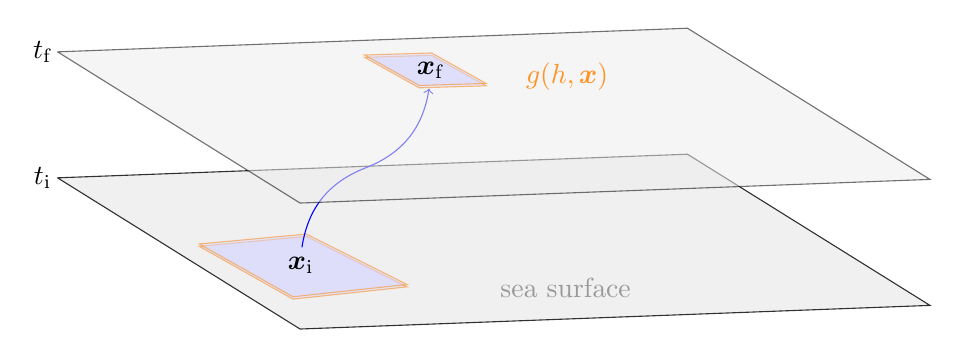
\begin{tikzpicture}

	% two planes
	\draw[fill=gray!15, opacity=0.8]\planemaina{-0.8}{$t_{\textrm{i}}$}{sea surface};
	
	\draw[orange, fill=blue!15, opacity=0.5]\planelittlea{-1.67};
	\draw[orange, fill=blue!15, opacity=0.5]\planelittlea{-1.64};
			
	\path (-0.45,-3.45,-2) node (x) {$\boldsymbol{x}_{\textrm{i}}$} 
	(1,-1.17,-2.5) node (y) {$\boldsymbol{x}_{\textrm{f}}$};
	
    \draw[-{>[scale=1.25]},blue] (x) to [bend left=30] ($(x)!0.5!(y)$) to [bend right=30] (y); 
    
	\draw[fill=gray!15, opacity=0.55]\planemainb{0.8}{$t_{\textrm{f}}$}{$g(h,\boldsymbol{x})$};
	
    \draw[orange, fill=blue!15, opacity=0.5]\planelittlec{0.73};
    \draw[orange, fill=blue!15, opacity=0.5]\planelittlec{0.76};
	
	\node at (y) {$\boldsymbol{x}_{\textrm{f}}$};

\end{tikzpicture}
\end{figure}

\begin{equation*}
	{\int_{t_{\textrm{i}}}^{t_{\textrm{f}}}}\;\int_{A}\;
	\Big(\nabla\cdot \bar{\pmb{\sigma}} -m\,\frac{d\dot{\pmb{x}}}{dt} \Big)
	\cdot\delta{\pmb{x}}\;dA\;dt=0
\end{equation*}

\end{frame}



%%%%%%%%%% section 2: Non-Conservative Action %%%%%%%%%% 

\section{Non-Conservative Stationary Ridging Action}

\begin{frame}
\frametitle{\insertsection}
\vspace{-5mm}
\begin{equation*}
\mathfrak{f}\colon\mathfrak{g}(h,\phi,s,\varepsilon,\pmb{x})\mapsto g(h,\phi_R,\pmb{x})
\end{equation*}
\vspace{-7mm}
\begin{figure}[h]
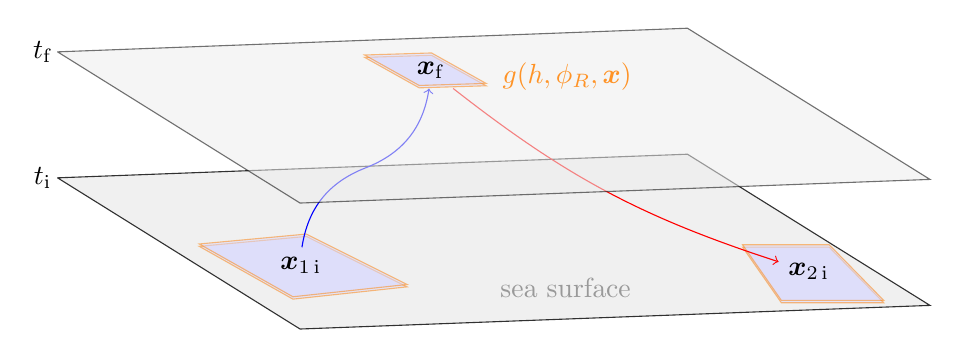
\begin{tikzpicture}

	% two planes
	\draw[fill=gray!15, opacity=0.8]\planemaina{-0.8}{$t_{\textrm{i}}$}{sea surface};
	
	\draw[orange, fill=blue!15, opacity=0.5]\planelittlea{-1.67};
	\draw[orange, fill=blue!15, opacity=0.5]\planelittlea{-1.64};
	
	\draw[orange, fill=blue!15, opacity=0.5]\planelittleb{-1.68};
	\draw[orange, fill=blue!15, opacity=0.5]\planelittleb{-1.65};
		
	\path (-0.45,-3.45,-2) node (x) {$\boldsymbol{x}_{1\,\textrm{i}}$} 
	(1,-1.17,-2.5) node (y) {$\boldsymbol{x}_{\textrm{f}}$} 
	(6,-3.53,-2) node (z) {$\boldsymbol{x}_{2\,\textrm{i}}$};
	
    \draw[-{>[scale=1.25]},blue] (x) to [bend left=30] ($(x)!0.5!(y)$) to [bend right=30] (y); 
    \draw[-{>[scale=1.25]},red] (y) to [bend right=10] (z); 
    
	\draw[fill=gray!15, opacity=0.55]\planemainb{0.8}{$t_{\textrm{f}}$}{$g(h,\phi_R,\boldsymbol{x})$};
	
    \draw[orange, fill=blue!15, opacity=0.5]\planelittlec{0.73};
    \draw[orange, fill=blue!15, opacity=0.5]\planelittlec{0.76};
	
	\node at (y) {$\boldsymbol{x}_{\textrm{f}}$};

\end{tikzpicture}
\end{figure}
\vspace{-2mm}
\begin{equation*}
	\mathcal{S}[\pmb{x}_1,\pmb{x}_2]=\int_{t_{\textrm{i}}}^{t_{\textrm{f}}}\;\int_{A}\;\Omega[\pmb{x}_1,\pmb{x}_2]\;dA\;dt
\end{equation*}

\scriptsize{Galley, C. R., D. Tsang, and L. C. Stein (2014), The principle of stationary nonconservative action for classical mechanics and field theories, arXiv:1412.3082}

\end{frame}

\begin{frame}
\frametitle{\insertsection}

\begin{figure}[h]
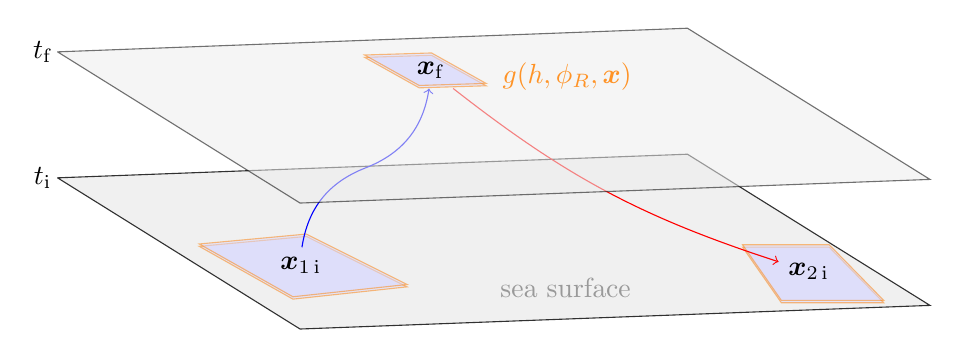
\begin{tikzpicture}

	% two planes
	\draw[fill=gray!15, opacity=0.8]\planemaina{-0.8}{$t_{\textrm{i}}$}{sea surface};
	
	\draw[orange, fill=blue!15, opacity=0.5]\planelittlea{-1.67};
	\draw[orange, fill=blue!15, opacity=0.5]\planelittlea{-1.64};
	
	\draw[orange, fill=blue!15, opacity=0.5]\planelittleb{-1.68};
	\draw[orange, fill=blue!15, opacity=0.5]\planelittleb{-1.65};
		
	\path (-0.45,-3.45,-2) node (x) {$\boldsymbol{x}_{1\,\textrm{i}}$} 
	(1,-1.17,-2.5) node (y) {$\boldsymbol{x}_{\textrm{f}}$} 
	(6,-3.53,-2) node (z) {$\boldsymbol{x}_{2\,\textrm{i}}$};
	
    \draw[-{>[scale=1.25]},blue] (x) to [bend left=30] ($(x)!0.5!(y)$) to [bend right=30] (y); 
    \draw[-{>[scale=1.25]},red] (y) to [bend right=10] (z); 
    
	\draw[fill=gray!15, opacity=0.55]\planemainb{0.8}{$t_{\textrm{f}}$}{$g(h,\phi_R,\boldsymbol{x})$};
	
    \draw[orange, fill=blue!15, opacity=0.5]\planelittlec{0.73};
    \draw[orange, fill=blue!15, opacity=0.5]\planelittlec{0.76};
	
	\node at (y) {$\boldsymbol{x}_{\textrm{f}}$};

\end{tikzpicture}
\end{figure}
\vspace{-10mm}
\begin{center}
\begin{equation*}
	\mathcal{S}[\pmb{x}_1,\pmb{x}_2]=\int_{t_{\textrm{i}}}^{t_{\textrm{f}}}\;\int_{A}\;\Omega[\pmb{x}_1,\pmb{x}_2]\;dA\;dt
\end{equation*}
For the non-conservative Lagrangian:
\begin{equation*}
\Omega[\pmb{x}_1,\pmb{x}_2] =\mathcal{L}(\pmb{x}_1,{\partial_\chi\pmb{x}_1},\pmb{X},t) -
	\mathcal{L}(\pmb{x}_2,{\partial_\chi\pmb{x}_2},\pmb{X},t)
	 + \mathcal{K}(\pmb{x}_1,\pmb{x}_2,{\partial_\chi\pmb{x}_1},{\partial_\chi\pmb{x}_2},\pmb{X},t)
\end{equation*}
\color{blue}Conservative Lagrangian $\mathcal{L}=\mathcal{T}-\mathcal{V}$\color{black}, \color{red}Non-Conservative Potential $\mathcal{K}$\color{black}
\end{center}

\end{frame}


%%%%%%%%%% section 3: Coarse-Grained Morphology %%%%%%%%%% 

\section{Coarse-Grained Ridge Morphology}

\begin{frame}
\frametitle{\insertsection}
\begin{columns}[T] % align columns
\begin{column}{.48\textwidth}
\begin{figure}[ht]
\noindent\centerline{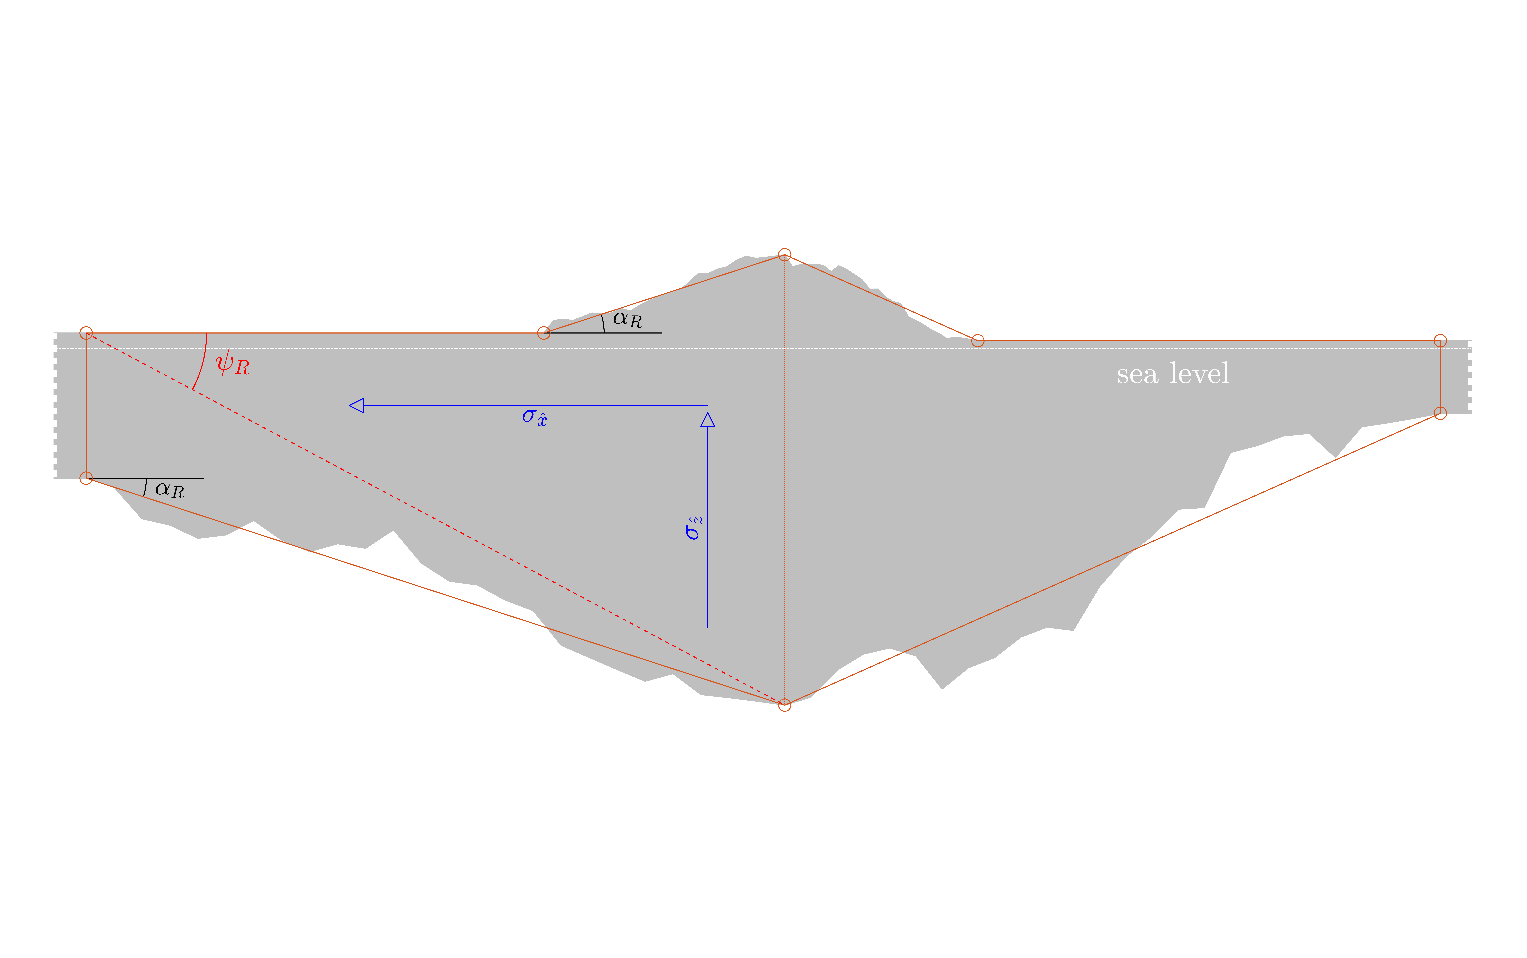
\includegraphics[width=0.8\textwidth,height=\textheight,keepaspectratio]{Figures/Friction_Model_Diagram.eps}}
%\caption{THis is a test}
\end{figure}
\end{column}%
\begin{column}{.48\textwidth}
\begin{minipage}[c][0.9\textheight][c]{\linewidth}
System of 14 equations:
\begin{itemize}
	\item Archimedes' Principle
	\item Conservation of Volume
	\item Conservation of Mass
	\item Geometric Constraints
	\item Highly Permeable Material
\end{itemize}
Boundary conditions: 
\begin{itemize}
	\item $h_{Fi}$, $h_{Fs}$, $\theta_R$
\end{itemize}
State variables:  
\begin{itemize}
	\item $\epsilon_{R_I}$, $\alpha_R$, $\phi_R$
\end{itemize}
\end{minipage}
\end{column}%
\end{columns}
\end{frame}


\begin{frame}
\frametitle{\insertsection}
\centering
Comparison with submarine data
\begin{figure}[ht]
\noindent\centerline{\includegraphics[width=0.8\textwidth,height=\textheight,keepaspectratio]{Figures/Davis_Wadhams_Comparison.eps}}
\caption{}
\end{figure}
\end{frame}

\begin{frame}
\frametitle{\insertsection}
\centering
Effect of strain $\epsilon_{R_I}$ and porosity $\phi_{R}$
\begin{figure}[ht]
\noindent\centerline{\includegraphics[width=\textwidth,height=\textheight,keepaspectratio]{Figures/Comparison_Diagram1.png}}
\label{fig:Comparison_Diagram1}
\end{figure}
The effect of changing $\phi_R$ from 0 to 0.2 is a 78\% expansion in ridge width, and 38\% inflation in keel depth. Therefore representing porosity in the dynamical core of sea ice models is important for representing form drag and fast ice.
\end{frame}


\begin{frame}
\frametitle{\insertsection}
\centering
Effect of strain $\epsilon_{R_I}$ and porosity $\phi_{R}$
\begin{figure}[ht]
\noindent\centerline{\includegraphics[width=0.8\textwidth,height=\textheight,keepaspectratio]{Figures/Thickness_DistR.eps}}
%\caption{$h_{F}=2.0$\,m and snow cover $h_{Fs}=0.3$\,m}
\end{figure}
\end{frame}


%%%%%%%%%% section 4: Coarse-Grained Mechanics %%%%%%%%%% 

\section{Coarse-Grained Ridge Mechanics}


\begin{frame}
\frametitle{\insertsection}
\centering
Applying the principle of non-conservative stationary action gives:
\begin{equation*}
0={\int_{t_{\textrm{i}}}^{t_{\textrm{f}}}}\;\int_{A}\;
	\bigg( {K_{p_1}}\,\delta\mathcal{V}_1
  - {K_{p_2}}\,\delta\mathcal{V}_2 \bigg)
  	\;dA\;dt 
\end{equation*}
Virtual potential energy along each path $\delta\mathcal{V}_{1,2}$ \\
Coefficients of Passive Stress ${K_{p_{1,2}}}$ along each path \\
\vspace{5mm}
In the physical limit of $\delta\mathcal{V}_{1}\to\delta\mathcal{V}_{2}$, ${K_{p_1}}\to{K_{p_2}}$ is constant, \\
which occurs when the following condition is met:
\begin{equation*}
\frac{\partial\sigma_{\hat{x}}}{\partial\alpha_R}=0
\end{equation*}
In this circumstance, ${K_{p}}=3$. Compare this with Hopkins et al. (1991), who obtained the range  $2.4\leq{K_{p}}\leq4.6$ with finite element modeling.

\end{frame}

\begin{frame}
\frametitle{\insertsection}
\centering
State space of ridges
\begin{figure}[ht]
\noindent\centerline{\includegraphics[width=0.8\textwidth,height=\textheight,keepaspectratio]{Figures/revised_manifold.png}}
\end{figure}
\end{frame}

\begin{frame}
\frametitle{\insertsection}
\centering
Ridge states with identical energetics (from previous slide)
\begin{figure}[ht]
\noindent\centerline{\includegraphics[width=0.8\textwidth,height=\textheight,keepaspectratio]{Figures/Expected_Plane.png}}
\end{figure}
\end{frame}

\begin{frame}
\frametitle{\insertsection}
\centering
Finding a path through the $\epsilon_{R_I}$ and $\phi_R$ state space.
\begin{equation*}
0={\int_{t_{\textrm{i}}}^{t_{\textrm{f}}}}\;\int_{A}\;
 	\bigg(\frac{\partial\sigma_{\hat{x}}}{\partial{\epsilon_{R_I}}}
 	      + \frac{\partial\sigma_{\hat{x}}}{\partial{\phi_{R}}} \frac{\partial{\phi_{R}}}{\partial{\epsilon_{R_I}}}
 	      + \cancelto{0}{\frac{\partial\sigma_{\hat{x}}}{\partial{\alpha_{R}}}} \frac{\partial{\alpha_{R}}}{\partial{\epsilon_{R_I}}}\bigg) \delta{\epsilon_{R_I}} \;dA\;dt 
\end{equation*}

\begin{figure}[ht]
\noindent\centerline{\includegraphics[width=0.6\textwidth,height=\textheight,keepaspectratio]{Figures/test.png}}
\label{fig:Stress_Annotation}
\end{figure}

\end{frame}

\begin{frame}
\frametitle{\insertsection}
\centering
Derived distributions from the Coarse-Grain Model
\begin{figure}[h]
\includegraphics[width=\textwidth,height=0.8\textheight,keepaspectratio]{Figures/Ridge_Formation_Probability.png}
\end{figure}
\end{frame}

\begin{frame}
\frametitle{\insertsection}
\centering
Derived distributions from the Coarse-Grain Model
\begin{figure}[h]
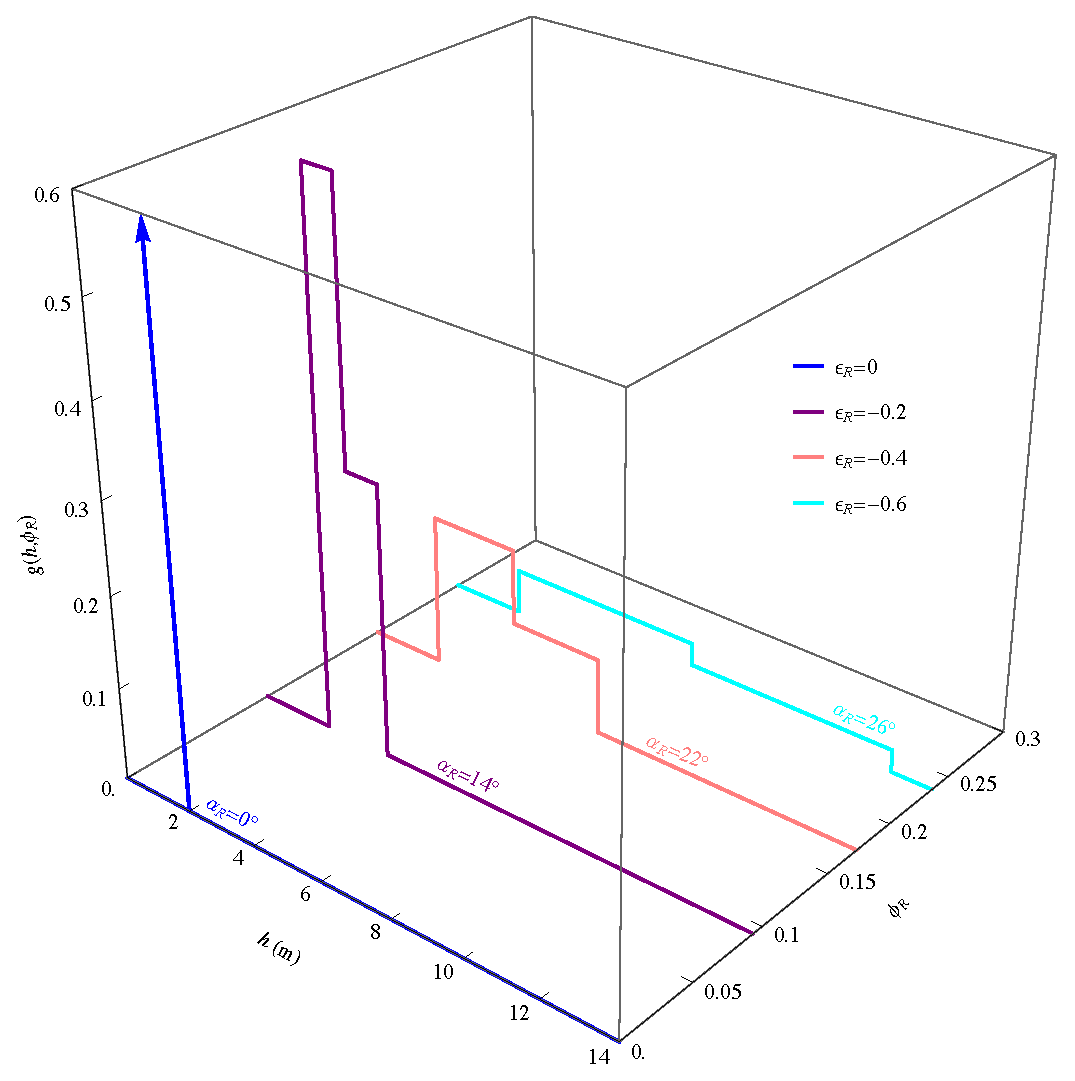
\includegraphics[width=\textwidth,height=0.8\textheight,keepaspectratio]{Figures/single_ridge_redistribution.eps}
\end{figure}
\end{frame}


{
\usebackgroundtemplate{
\parbox[c][\paperheight][c]{\paperwidth}{\centering\includegraphics[width=\paperwidth]{Figures/SEDNA_site1_3_20070409054800.jpg}}
}
\setbeamertemplate{footline}{}
\begin{frame}[t,fragile]

\begin{columns} % align columns
\begin{column}{0.5\textwidth}
\begin{figure}[h]
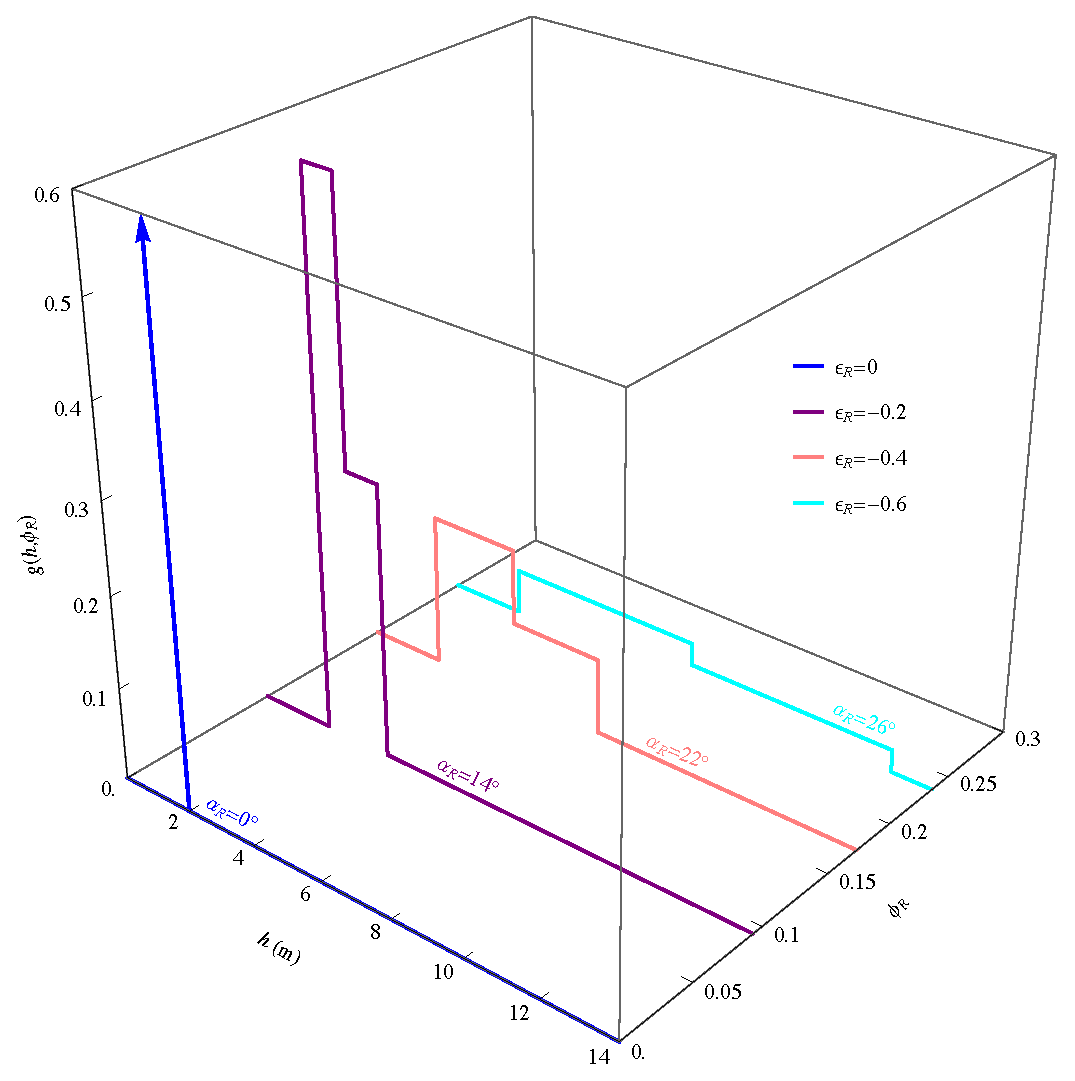
\includegraphics[width=\textwidth,height=0.8\textheight,keepaspectratio]{Figures/single_ridge_redistribution.eps}
\end{figure}
\end{column}
\begin{column}{.5\textwidth}
\centering
\color{white}
\Large
\begin{equation*}
m=\rho \int\limits_0^\infty g(h)\; h\; dh
\end{equation*}
\end{column}
\end{columns}
\end{frame}
}


\begingroup
\setbeamercolor{background canvas}{bg=black}
\begin{frame}
\frametitle{\color{white} Conclusions}

\begin{itemize}
  \item[\textcolor{white}{\textbullet}] \color{white} By considering sea ice ridging at the level of the action, rather than in Newton's second law, new insights become possible.
  \item[\textcolor{white}{\textbullet}] \color{white} A simple coarse-grained model is able to reproduce many desired features of ridges due to the underlying stationary assumption.
  \item[\textcolor{white}{\textbullet}] \color{white} Using this method, we are able to replace $g(h,\pmb{x})$ with $g(h,\phi_R,\pmb{x})$ to represent macro-porosity of sea ice of $A(\pmb{x})$.
  \item[\textcolor{white}{\textbullet}] \color{white} We do not presume that all sea ice is isostatic.
  \item[\textcolor{white}{\textbullet}] \color{white} The method provides new equations for redistribution $\Psi$ and compressive strength $P$ based on first principles.
  \item[\textcolor{white}{\textbullet}] \color{white} The next stage of this work is to apply it to CICE.
\end{itemize}
\end{frame}
\endgroup

\begingroup
\setbeamercolor{background canvas}{bg=black}
\setbeamertemplate{footline}{}
\begin{frame}
\begin{columns} % align columns
\begin{column}{0.3\textwidth}
\includegraphics[height=\textheight,keepaspectratio]{Figures/Europa.jpg}
\end{column}
\begin{column}{0.6\textwidth}
\begin{itemize}
	\item[] \color{white} \Large Office of Naval Research
	\item[] \color{white} \Large Department of Energy
	\item[] \color{white} \Large National Science Foundation
	\item[] ~
	\item[] \color{white} \scriptsize With thanks to Christopher Horvat, Adrian Turner, Jennifer Hutchings, Jackie Richter-Menge and Peter Wadhams. 
	\item[] ~
	\item[] \color{white} \Large afrobert@nps.edu
\end{itemize}
\end{column}
\end{columns}
\end{frame}
\endgroup



%%%%%%%%%%%%% SPARES %%%%%%%%%%%%%%%%%%%%%%%%

%\begin{frame}
%\frametitle{test2}
%\end{frame}


\end{document}
